\documentclass{article}

\usepackage[normalem]{ulem}
\usepackage{fancyhdr}
\usepackage[parfill]{parskip}
\usepackage{tikz}
\usepackage{multicol}
\pagestyle{fancyplain}
\usetikzlibrary{shapes, patterns}

\title{Photosynthesis}
\author{Todd Davies}
\date{\today}

\begin{document}

\rhead{Respiration}
\lhead{\today}

\maketitle

\section*{The stages of respiration}
\thispagestyle{empty}
Respiration releases the energy stored in glucose by oxidising it and creates ATP.

There are four stages of respiration, glycolysis, the link reaction, the Krebs cycle, and the electron transport chain.

\subsection*{Glycolysis}
Gylcolysis takes place in the cytoplasm of the cell. It is the only part of respiration that can function without oxygen.

Since sugars are unreactive, two molecules of ATP are used to add two phosphate groups to the glucose molecule, which is then broken down into two molecules of TP (triose phospoate). The TP is then oxidised to pyruvate and reduced NAD. This releases enough energy to create four ATP molecules from four ATP + pi molecules.

Since two ATP molecules were used to start the reaction, there is a \textbf{net gain of two ATP} molecules.

Here is a diagram of glycolysis:

\begin{center}
	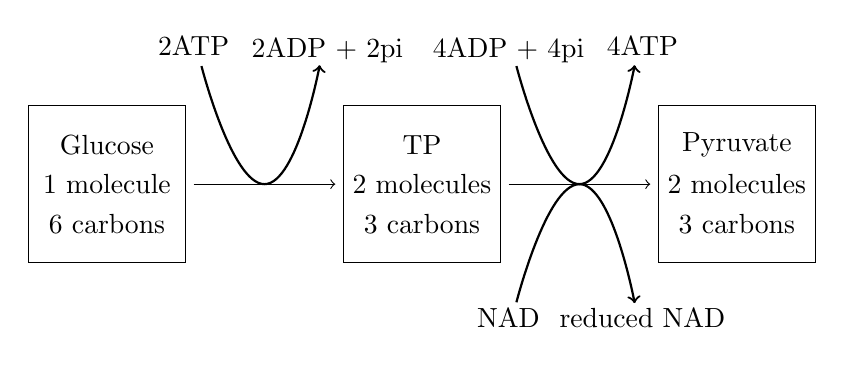
\begin{tikzpicture}
	%Glucose
		\draw (0,0) rectangle (2,2);
		\node at (1,1.5) {Glucose};
		\node at (1,  1) {1 molecule};
		\node at (1,0.5) {6 carbons};
	%Glucose->TP
		\draw[->] (2.1,1) -- (3.9,1);
	%ATP->ADP + pi
		\draw[thick] plot [smooth,tension=1] coordinates{(2.2, 2.5) (3, 1) (3.7, 2.5)};
		\draw [thick, ->] (3.7, 2.5) -- (3.701, 2.51);   %Right
		\node at (2.1, 2.75) {2ATP};
		\node at (3.8, 2.7) {2ADP + 2pi};
	%TP
		\draw (4,0) rectangle (6,2);
		\node at (5,1.5) {TP};
		\node at (5,  1) {2 molecules};
		\node at (5,0.5) {3 carbons};
	%TP->Pyruvate
		\draw[->] (6.1,1) -- (7.9,1);
	%ADP+pi->ATP
		\draw[thick] plot [smooth,tension=1] coordinates{(6.2, 2.5) (7, 1) (7.7, 2.5)};
		\draw [thick, ->] (7.7, 2.5) -- (7.701, 2.51);   %Right
		\node at (6.1, 2.7) {4ADP + 4pi};
		\node at (7.8, 2.75) {4ATP};
	%NAD->reduced NAD
		\draw[thick] plot [smooth,tension=1] coordinates{(6.2, -0.5) (7, 1) (7.7, -0.5)};
		\draw [thick, ->] (7.7, -0.5) -- (7.701, -0.51);   %Right
		\node at (6.1, -0.7) {NAD};
		\node at (7.8, -0.7) {reduced NAD};
	%Pyruvate
		\draw (8,0) rectangle (10,2);
		\node at (9,1.5) {Pyruvate};
		\node at (9,  1) {2 molecules};
		\node at (9,0.5) {3 carbons};
	\end{tikzpicture}
\end{center}

\end{document}